\chapter{Using Capacitors}

We have connected out capacitor to a triangular voltage source and a resistor. The circuit is shown in Figure \ref{fig:triangular-circuit}.

\begin{figure}[h]
    \centering
    \begin{circuitikz} \draw
        (0,0) to[triangle voltage source] (0,4)
        to[R, l=$5k\Omega$] (4,4) 
        to[C, l=C] (4,0) -- (0,0)
        ;
        \end{circuitikz}
    \caption{Circuit with Triangular Voltage Source \& Capacitor}
    \label{fig:triangular-circuit}
\end{figure}

The voltage source is a triangular wave with a peak-to-peak voltage of 5V and a frequency of 50kHz.

\section{Triangular Wave in Fourier Series}

According to \cite{wolfram_triangle_wave} from WolframAlpha, The triangular wave can be represented as a Fourier series. The Fourier series of a triangular wave is given by:

\begin{align*}
    V(t) &= \frac{8V_{pp}}{\pi^2} \sum_{n=1,3,5,\ldots}^{\infty} \frac{(-1)^{\frac{n-1}{2}}}{n^2} \sin(2\pi n f t)
\end{align*}

where $V_{pp}$ is the peak-to-peak voltage of the wave, $f$ is the frequency of the wave, and $t$ is the time. So, our triangular wave can be represented as:

\begin{align*}
    V(t) &= \frac{8 \times 5}{\pi^2} \sum_{n=1,3,5,\ldots}^{\infty} \frac{(-1)^{\frac{n-1}{2}}}{n^2} \sin(2\pi n \times 50 \times 10^3 t)
\end{align*}

\newpage
\thispagestyle{plain}

\section{Measuring the Output Voltage}

We have connected the circuit to an oscilloscope to measure the output voltage across the capacitor. The output voltage is shown in Figure \ref{fig:triangular-output}.

\begin{figure}[h]
    \centering
    \includegraphics[width=0.6\textwidth]{assets/WhatsApp Image 2024-04-16 at 18.20.11 (3).jpeg}
    \caption{Triangular Wave Input Voltage}
    \label{fig:triangular-input}
\end{figure}


\begin{figure}[h]
    \centering
    \includegraphics[width=0.6\textwidth]{assets/WhatsApp Image 2024-04-16 at 18.20.11 (1).jpeg}
    \caption{Output Voltage Across Capacitor}
    \label{fig:triangular-output}
\end{figure}

As we can see, when we connect a triangular wave to a capacitor, the output voltage is tends to act like a sine wave. This is because the capacitor charges and discharges according to the input voltage. The output voltage is the voltage across the capacitor, which is the integral of the input voltage.

\newpage
\thispagestyle{plain}

\subsection{FFT Analysis}

\subsubsection{FFT of Triangular Wave}

To analyze the output voltage, we can use the Fast Fourier Transform (FFT) to find the frequency components of the signal. The FFT of the triangular wave is shown in Figure \ref{fig:triangular-fft}.

\begin{figure}[h]
    \centering
    \includegraphics[width=1\textwidth]{assets/triangular-fft.jpg}
    \caption{FFT of Triangular Wave}
    \label{fig:triangular-fft}
\end{figure}

We can see the FFT result as the purple graph in Figure \ref{fig:triangular-fft}.

\begin{itemize}
    \item A triangular waveform is composed of multiple harmonics, with the fundamental frequency being the lowest.
    \item When you apply FFT to a triangular wave, you'll see a dominant peak at the fundamental frequency, and smaller peaks at integer multiples of the fundamental frequency (harmonics).
    \item The FFT plot shows a series of peaks, with the tallest peak at the fundamental frequency and decreasing peak heights for each harmonic. 
\end{itemize}

\newpage
\thispagestyle{plain}

\subsubsection{FFT of Sinusoidal Wave}

The FFT of the sinusoidal wave is shown in Figure \ref{fig:sinusoidal-fft}.

\begin{figure}[h]
    \centering
    \includegraphics[width=1\textwidth]{assets/sinusodial-fft.jpeg}
    \caption{FFT of Sinusoidal Wave}
    \label{fig:sinusoidal-fft}
\end{figure}

We can see the FFT result as the purple graph in Figure \ref{fig:sinusoidal-fft}.

\begin{itemize}
    \item A sinusoidal waveform consists of a single frequency component.
    \item When you apply FFT to a sinusoidal wave, you will see a sharp peak at the frequency of the sinusoid, with very little energy elsewhere.
    \item The FFT plot will have a single prominent peak corresponding to the frequency of the sinusoidal wave.
\end{itemize}

\newpage
\thispagestyle{plain}

\subsubsection{FFT of Triangular Wave Across Capacitor}
The FFT of the triangular wave fed to the capacitor is shown in Figure \ref{fig:triangular-fft-capacitor}.

\begin{figure}[h]
    \centering
    \includegraphics[width=1\textwidth]{assets/triangular-fft-capacitor.jpg}
    \caption{FFT of Triangular Wave Across Capacitor}
    \label{fig:triangular-fft-capacitor}
\end{figure}

We can see the FFT result as the purple graph in Figure \ref{fig:triangular-fft-capacitor}.

\begin{itemize}
    \item Adding a capacitor to a triangular waveform can result in a smoother waveform, \textbf{akin to filtering out some of the higher frequency harmonics.} 
    \item The capacitor smoothens out the edges of the triangular waveform, reducing the steepness of the transitions.
    \item When you apply FFT to a triangular wave with a capacitor, you'll see a dominant peak at the fundamental frequency similar to the regular triangular wave, but with potentially reduced energy in the higher harmonics compared to the regular triangular wave.
    \item The FFT plot will still have multiple peaks, but the relative amplitudes of the harmonics might be different compared to the regular triangular wave.
\end{itemize}

\newpage
\thispagestyle{plain}

\subsection{Circuit Analysis}

To analyze the circuit with a constant voltage \( V \) applied and initially uncharged capacitor, let's denote:

\begin{itemize}
    \item \( q(t) \) as the charge on the capacitor at time \( t \).
    \item \( V_C(t) \) as the voltage across the capacitor at time \( t \).
    \item \( V_R(t) \) as the voltage across the resistor at time \( t \).
    \item \( I(t) \) as the current flowing through the circuit at time \( t \).
    \item \( R \) as the resistance of the resistor.
    \item \( C \) as the capacitance of the capacitor.
\end{itemize}

The Kirchhoff loop rule for the circuit gives:

\[ V = V_R(t) + V_C(t) \]

Using Ohm's law \( V_R(t) = IR \) and \( I(t) = \frac{dq(t)}{dt} \), and the relationship between charge and voltage for a capacitor \( V_C(t) = \frac{q(t)}{C} \), we can rewrite the Kirchhoff loop equation as:

\[ V = IR + \frac{q(t)}{C} \]

Solving this for \( I \), we have:

\[ I = \frac{dq(t)}{dt} = \frac{V - \frac{q(t)}{C}}{R} \]

This is a first-order ordinary differential equation (ODE) that governs the charge on the capacitor \( q(t) \). We can solve it using standard techniques for solving ODEs.

To solve the ODE, we can separate variables and integrate both sides:

\[ \int \frac{dq}{V - \frac{q}{C}} = \int \frac{dt}{R} \]

\[ -C\ln\left|V - \frac{q}{C}\right| = \frac{t}{R} + K \]

where \( K \) is the constant of integration. Solving for \( q(t) \), we get:

\[ V - \frac{q}{C} = Ce^{-\frac{t}{RC}} \]

\[ q(t) = CV(1 - e^{-\frac{t}{RC}}) \]

This is the expression for the charge on the capacitor as a function of time \( t \) and the constants \( V \), \( C \), and \( R \). 

The resistance \( R \) affects the time constant of the charging process. A larger resistance \( R \) will slow down the rate at which the capacitor charges, leading to a slower rise in the charge \( q(t) \) over time. Conversely, a smaller resistance \( R \) will lead to a faster charging process. 

\newpage
\thispagestyle{plain}

Now, let's plot \( q(t) \) for certain numerical values of \( V \), \( C \), and \( R \). For example, let's take \( V = 10 \) volts, \( C = 1 \) farad, and \( R = 1,2,3 \) ohm. We can then plot \( q(t) \) over a range of time.

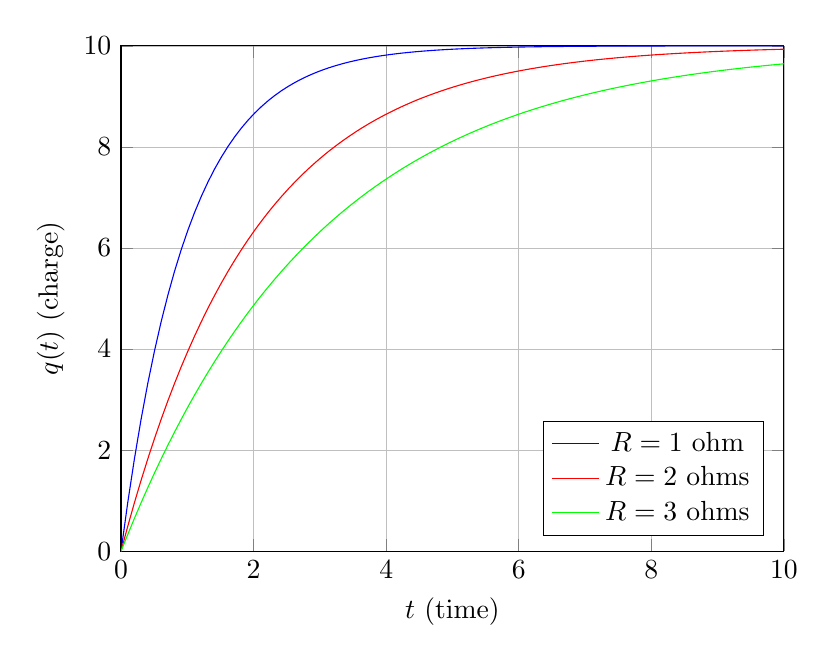
\begin{tikzpicture}
    \begin{axis}[
        xlabel={$t$ (time)},
        ylabel={$q(t)$ (charge)},
        xmin=0, xmax=10,
        ymin=0, ymax=10,
        xtick={0,2,4,6,8,10},
        ytick={0,2,4,6,8,10},
        legend pos=south east,
        grid=both,
        grid style={line width=.1pt, draw=gray!10},
        major grid style={line width=.2pt,draw=gray!50},
        width=10cm,
        height=8cm
    ]
    
    \addplot[
        domain=0:10,
        samples=100,
        color=blue,
        ]
        {10*(1 - exp(-x))};
    \addlegendentry{$R = 1$ ohm}
    
    \addplot[
        domain=0:10,
        samples=100,
        color=red,
        ]
        {10*(1 - exp(-x/2))};
    \addlegendentry{$R = 2$ ohms}
    
    \addplot[
        domain=0:10,
        samples=100,
        color=green,
        ]
        {10*(1 - exp(-x/3))};
    \addlegendentry{$R = 3$ ohms}
    
    \end{axis}
    \end{tikzpicture}

\subsection{Convergence Analysis}

To find the corresponding sequence \( q_{\text{max},n} \) for the maximum charge of the capacitor as a function of \( R_n = nR \), we need to consider the charging curve \( q(t) \) for each \( R_n \) and find the maximum value of \( q(t) \).

From our previous analysis, we know that the charge on the capacitor as a function of time \( t \) for a given \( R \) is given by:

\[ q(t) = CV(1 - e^{-\frac{t}{RC}}) \]

For \( R_n = nR \), the charge function becomes:

\[ q_n(t) = CV(1 - e^{-\frac{t}{nRC}}) \]

To find the maximum charge, we need to find the maximum value of \( q_n(t) \). This occurs when \( e^{-\frac{t}{nRC}} = 0 \), which happens when \( \frac{t}{nRC} = \infty \), or equivalently when \( t = \infty \). Therefore, the maximum charge \( q_{\text{max},n} \) occurs as \( t \) approaches infinity, which is:

\[ q_{\text{max},n} = CV \]

This implies that the maximum charge of the capacitor for each \( R_n \) is independent of \( R_n \), and it is solely determined by the initial voltage \( V \) and capacitance \( C \). Therefore, the sequence \( q_{\text{max},n} \) is a constant sequence, and it converges to the maximum charge \( q_{\text{max}} = CV \) as \( n \) approaches infinity.

Regarding the convergence of the infinite series \( q_{\text{max},n} \), since it is a constant sequence, the series trivially converges to \( q_{\text{max}} = CV \) which means \textbf{sequence is convergent}. There's no need to investigate convergence properties further as the sequence is constant. \textbf{Series is divergent} because the terms do not approach zero and infinite sum tends to infinity.


